\subsection{Delegable Prove}\label{section: zk-zkvm-delegable-prove}

The Section \ref{section: zkzkvm-user-end-prove} scheme highlights a key challenge in generating cryptographic proofs for transactions in a blockchain network. As the complexity of the transaction and the number of calls involved increases, so does the cost of creating and including the proof in the transaction. This poses a significant problem for users, particularly those using weaker devices such as mobile phones or hardware tokens.

To address this issue, a solution called Delegable Prove Scheme (DPS) has been proposed. DPS allows users to delegate the task of generating cryptographic proofs to a third party in a privacy-preserving manner, such as a server or a more powerful device, while still maintaining the security and validity of the transaction. This means that users can conduct complex transactions without incurring the high cost of generating proofs themselves.

The key system and note design used in DPS ensures that transactions remain private and secure, even when proof generation is delegated to a third party. The system creates notes, which represent a certain unit of state, and each note is assigned a unique key. When a user wants to send a private transaction, they create a new note with a new stealth key and send it to the receiver. To ensure that the transaction is valid, a cryptographic proof is required to show that the note has not been previously spent or duplicated.

\subsubsection{Current design}

We compared the proof generation schemes of ZCash \cite{website:zcash-nu5}, ZEXE \cite{cryptoeprint:2018/962}, VERI-ZEXE \cite{cryptoeprint:2022/802}, Aleo \cite{website:aleo-vm}, Aztec3 \cite{website:Aztec3}, and Efficient Private Delegation of zkSNARK Provers \cite{website:epdzp} as shown in the diagram \ref{fig:cur_proof_generation} below:
\begin{figure}[!ht]
    \centering
    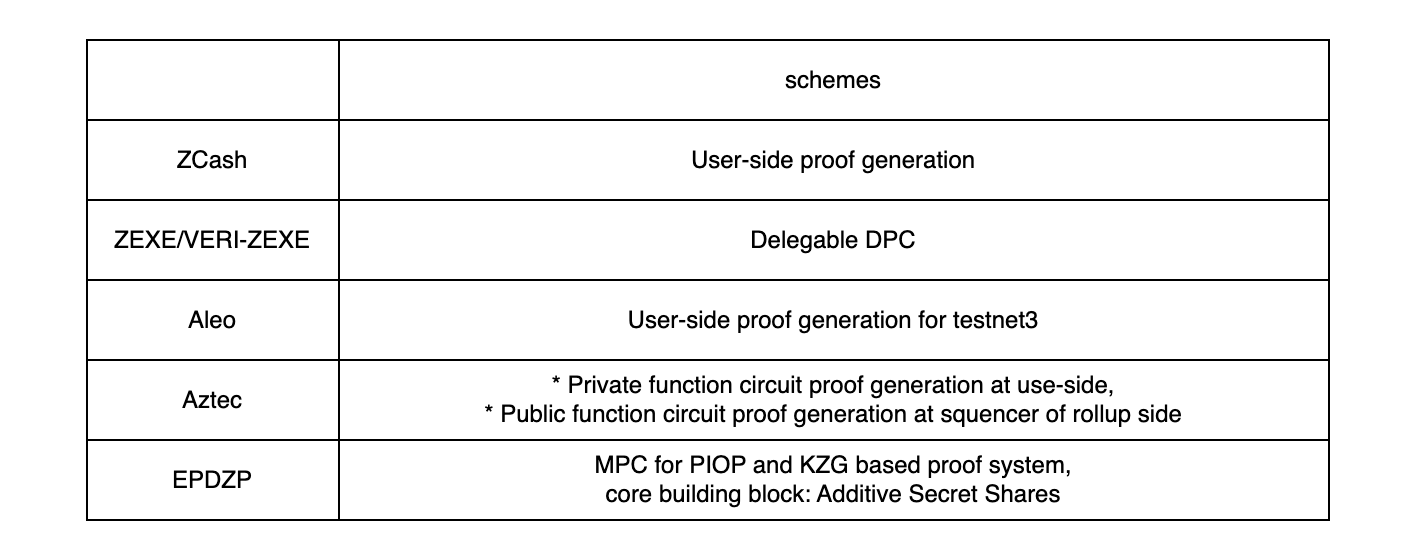
\includegraphics[width=0.6\textwidth]{cur proof generation.jpg}
    \caption{Current Proof Generation Schemes}
    \label{fig:cur_proof_generation}
\end{figure}

As we can see from above diagram, ZCash's proof generation scheme is user-side proof generation, which means ZCash has only one type of transaction, which is the transfer of ZEC. The transaction is not complex and the corresponding circuit size is not very large. Therefore, when it comes to proof generation, such as for shielded transactions, it can be done on the user side, for example, generating proofs within a wallet.

The delegable DPC protocol in ZEXE \cite{cryptoeprint:2018/962} allows for the delegation of computations while maintaining security. The protocol involves a delegator who sends input parameters to a delegatee, who then performs an offline computation and generates a proof of correctness using zero-knowledge proofs. The delegatee sends this proof along with the output of the computation back to the delegator, who can use it to generate a transaction that attests to the correctness of the computation. This transaction can be publicly verified by anyone without revealing any additional information about it.

To ensure privacy, ZEXE uses a combination of cryptographic techniques such as zero-knowledge proofs and randomizable signatures. The randomizable signature scheme is used to prevent linking across multiple signatures, which is important for maintaining security in the delegable DPC protocol that the delegatee can not impersonate the delegator, e.g., by producing further transactions that the delegator never authorized.

VERI-ZEXE and ZEXE use the same delegable DPC scheme, we will not repeat it. Aleo's current implementation (testnet3) is still user-side and uses SNARK-powered circuits to generate proofs, but does not yet implement delegable DPC.

Aztec3 \cite{website:Aztec3} uses a recursive circuit to generate the final proof, and each contract function is a circuit when a proof needs to be generated. The recursion uses two system circuits, private kernel circuits and public kernel circuits. All private related function calls and their proofs must be entered into private kernel circuits to generate proofs, while all public related function calls and their proofs must be entered into public kernel circuits to generate proofs. In short, the proof of the private circuit is generated on the client side, while the proof of the public circuit is generated in Rollup's Squencer.

Efficient Private Delegation of zkSNARK Provers \cite{website:epdzp} uses MPC to do outsouring proveing. While it keeps witness private and proving efficient, it is designed for Polynomial IOPs and MPC friendly polynomial commitments proof system, while our ZK-ZKVM uses Starky as its internal proof system, which is not suitable for it.

\subsubsection{Our work}

Our design based on ZEXE, and the main procedure of delegable transactions as shown in the diagram \ref{fig:delegable_tx} below:

\begin{figure}[!ht]
    \centering
    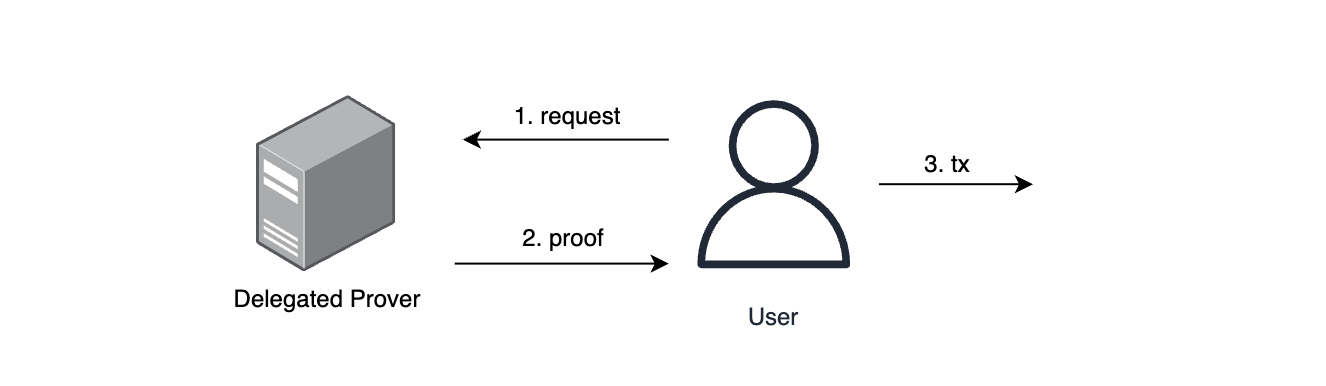
\includegraphics[width=0.6\textwidth]{delegable tx.jpg}
    \caption{Delegable transactions}
    \label{fig:delegable_tx}
\end{figure}

Although ZEXE does not allow the delegatee to impersonate the delegator, the witness remains visible to all participants on the public blockchain. This lack of privacy does not serve our purpose for ZK-ZKVM. To address this issue, we incorporated an external cryptographic primitive called the Secret Share Scheme.

We generate a shared secret by combining the delegatee's public key with the delegator's private key. We then use this shared key to symmetrically encrypt the witness on the delegator's side, and send the encrypted witness to the delegatee. The delegatee uses their private key and the delegator's public key to retrieve the shared key and decrypt the witness.

Once the witness data is decrypted, the subsequent process is identical to that of ZEXE.

Let's say User Alice is the delegator, Prover Bob is the delegatee. We briefly explain our delegable prove scheme:

\begin{itemize}
    \item Alice generates shared key $key_{shared} = sk_{alice} \cdot pk_{bob}$
    \item Alice encrypt the witness, the encrypted witness is $witness_{enc} = enc(key_{shared}, witness)$
    \item Alice send the encrypted witness to Bob, while other participants on the public blockchain knows nothing.
    \item Bob generates shared key $key_{shared}' = sk_{bob} \cdot pk_{alice}$, which is same as $key_{shared}$
    \item Bob decrypt the encrypted witness, get raw witness, $witness = dec(key_{shared}', witness_{enc})$
    \item Bob use decrypted witness generating proof $\pi$, send proof back to Alice.
    \item Alice uses her signature private key to construct a transaction within proofs, send it to the blockchain.
\end{itemize}

Our high-level description of our scheme as shown in the diagram \ref{fig:our_proof_generation} below:
\begin{figure}[!ht]
    \centering
    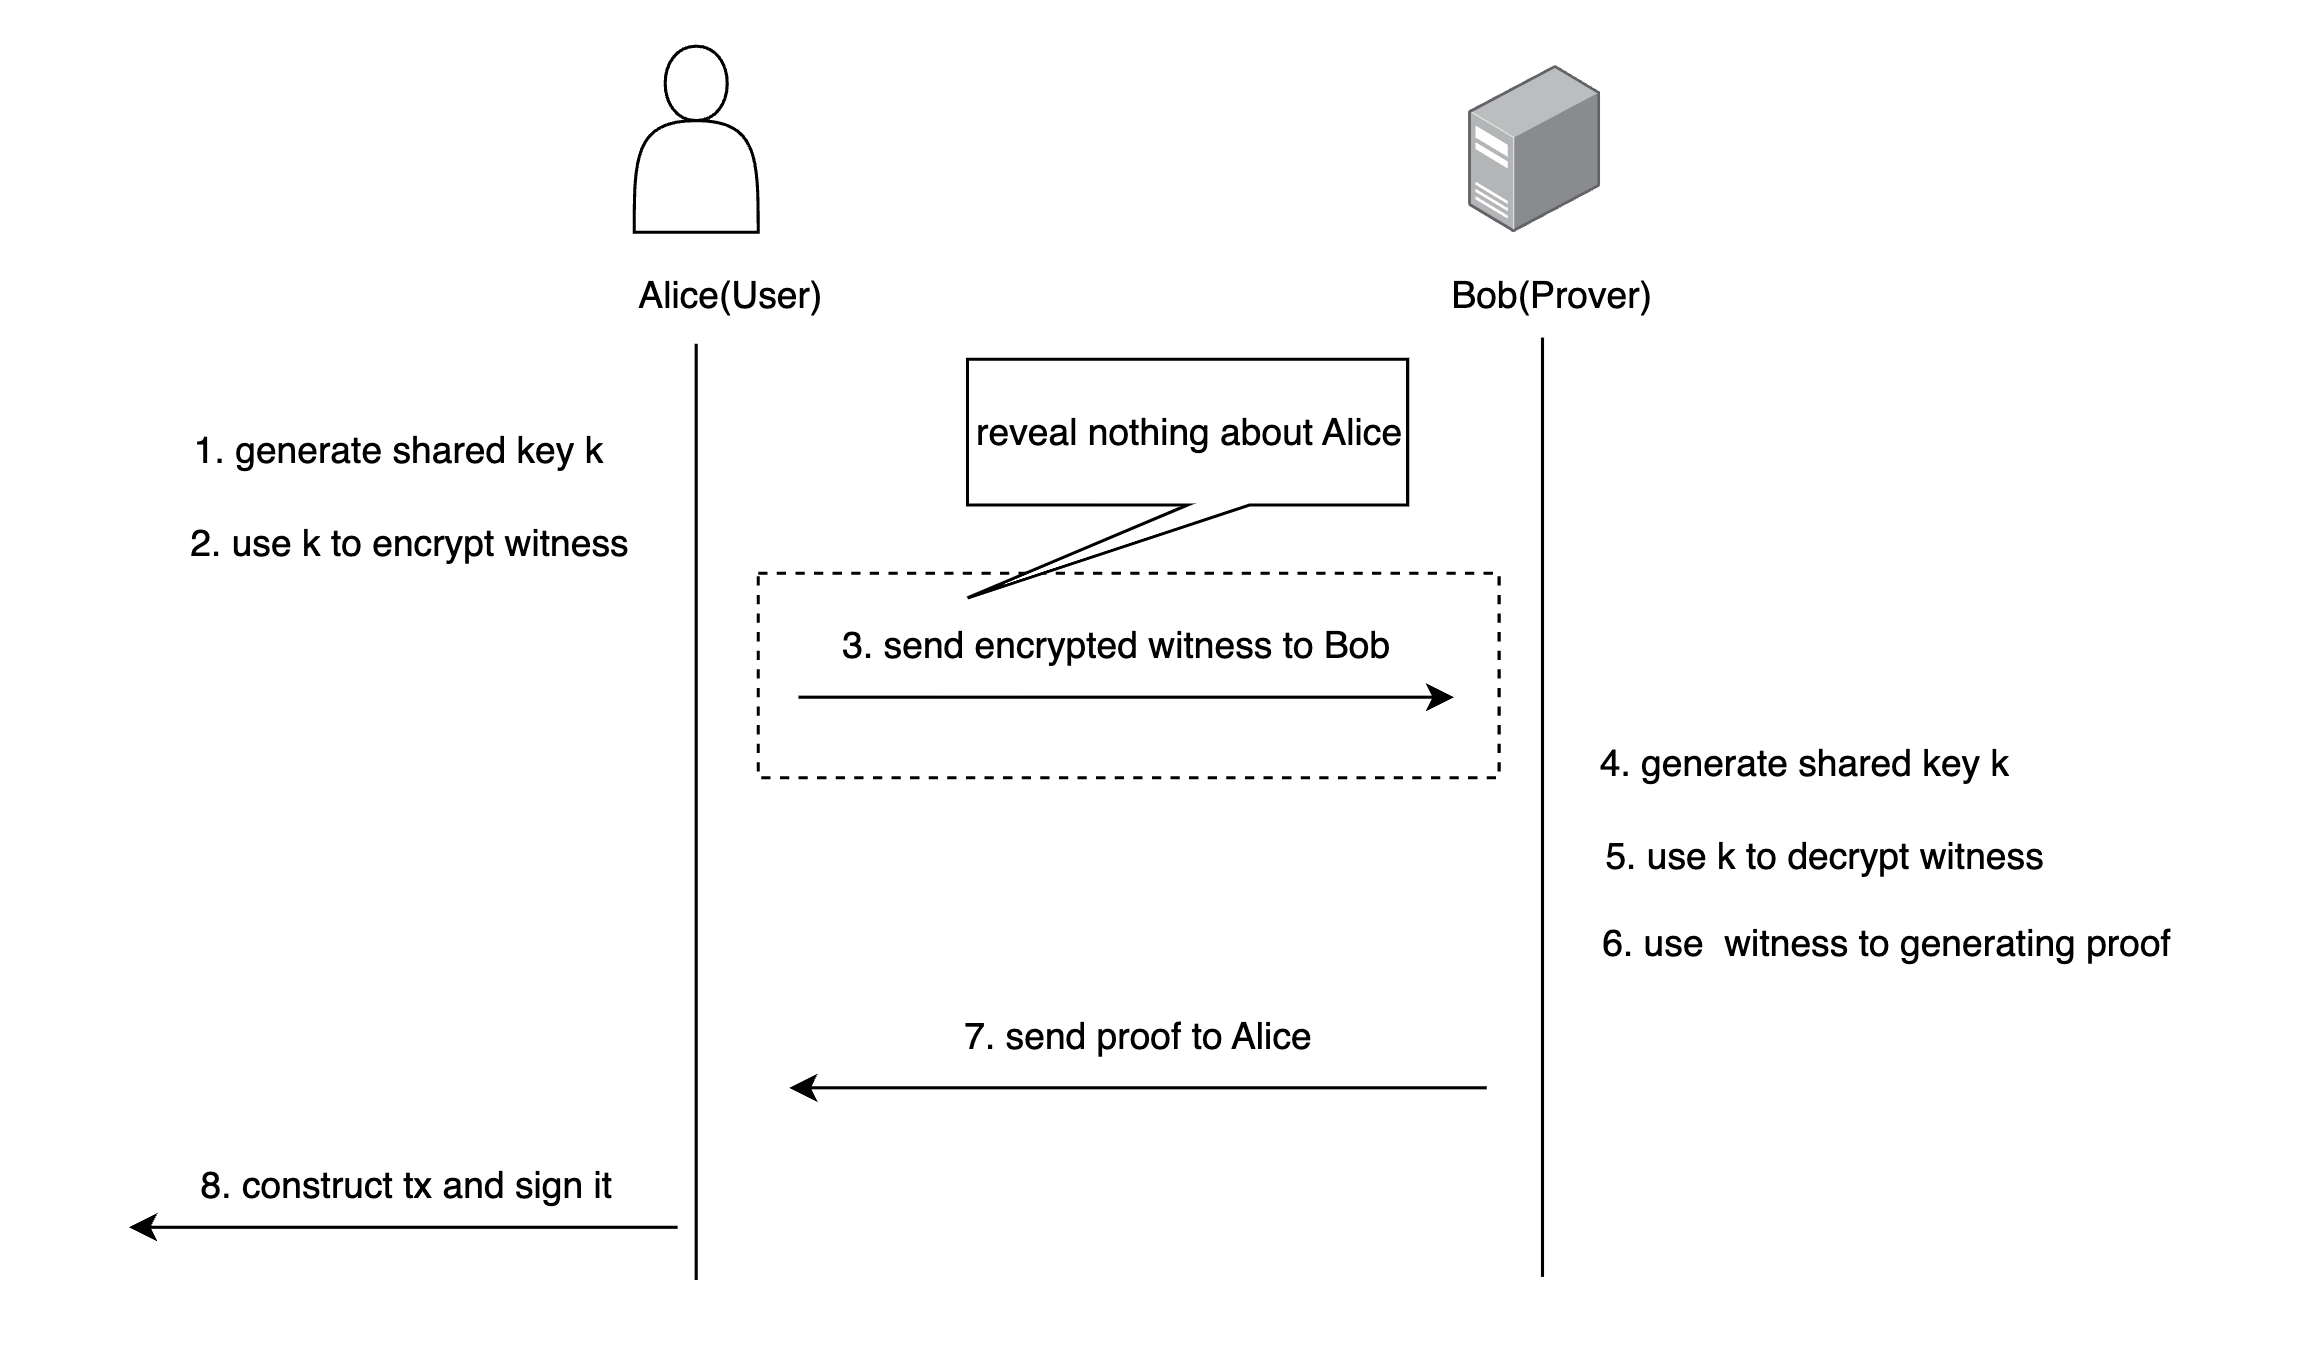
\includegraphics[width=0.6\textwidth]{our proof generation.jpg}
    \caption{Our Proof Generation Scheme}
    \label{fig:our_proof_generation}
\end{figure} 